%%%%%%%%%%%%%%%%%%%%%%%%%%%%%%%%%%%%%%%%%
% University Assignment Title Page 
% LaTeX Template
% Version 1.0 (27/12/12)
%
% This template has been downloaded from:
% http://www.LaTeXTemplates.com
%
% Original author:
% WikiBooks (http://en.wikibooks.org/wiki/LaTeX/Title_Creation)
%
% License:
% CC BY-NC-SA 3.0 (http://creativecommons.org/licenses/by-nc-sa/3.0/)
% 
% Instructions for using this template:
% This title page is capable of being compiled as is. This is not useful for 
% including it in another document. To do this, you have two options: 
%
% 1) Copy/paste everything between \begin{document} and \end{document} 
% starting at \begin{titlepage} and paste this into another LaTeX file where you 
% want your title page.
% OR
% 2) Remove everything outside the \begin{titlepage} and \end{titlepage} and 
% move this file to the same directory as the LaTeX file you wish to add it to. 
% Then add \input{./title_page_1.tex} to your LaTeX file where you want your
% title page.
%
%%%%%%%%%%%%%%%%%%%%%%%%%%%%%%%%%%%%%%%%%

%----------------------------------------------------------------------------------------
%	PACKAGES AND OTHER DOCUMENT CONFIGURATIONS
%----------------------------------------------------------------------------------------

\documentclass[12pt]{article}

% https://www.sharelatex.com/learn/Page_size_and_margins
\usepackage[a4paper, total={6in, 8in}]{geometry}
% Sizing and placement of images
\usepackage{graphicx}
\usepackage{float}
% For Code segments
\usepackage{listings}
% Add Colors for Scala code
\usepackage{xcolor}
% "define" Scala Colors
\usepackage[T1]{fontenc}
\usepackage{beramono}
\definecolor{dkgreen}{rgb}{0,0.6,0}
\definecolor{gray}{rgb}{0.5,0.5,0.5}
\definecolor{mauve}{rgb}{0.58,0,0.82}

\lstset{emph={%  
    val, sends, gotoStep, receives, forall, =>,branchOn, next%
    },emphstyle={\color{blue}}%
}%
%validate: String => Either[ValidationError, Any]
\lstdefinestyle{myScalastyle}{
  frame=tb,
  language=scala,
  aboveskip=3mm,
  belowskip=3mm,
  showstringspaces=false,
  columns=flexible,
  basicstyle={\small\ttfamily},
  numbers=none,
  numberstyle=\tiny\color{gray},
  keywordstyle=\color{blue},
  commentstyle=\color{dkgreen},
  stringstyle=\color{mauve},
  frame=single,
  breaklines=true,
  breakatwhitespace=true,
  tabsize=3,
}

\lstset{language=Java,
  showspaces=false,
  showtabs=false,
  breaklines=true,
  showstringspaces=false,
  breakatwhitespace=true,
  commentstyle=\color{pgreen},
  keywordstyle=\color{pblue},
  stringstyle=\color{pred},
  basicstyle=\ttfamily,
  moredelim=[il][\textcolor{pgrey}]{$$},
  moredelim=[is][\textcolor{pgrey}]{\%\%}{\%\%}
}

% Math tools - http://en.wikibooks.org/wiki/LaTeX/Mathematics
\usepackage{mathtools}
% Makes links
\usepackage{hyperref}
\hypersetup{
    colorlinks=true,
    citecolor=black,
    filecolor=black,
    linkcolor=black,
    urlcolor=black
}
\graphicspath{ {images/} }

\renewcommand{\baselinestretch}{1.1}


\begin{document}

\begin{titlepage}

\newcommand{\HRule}{\rule{\linewidth}{0.5mm}} % Defines a new command for the horizontal lines, change thickness here

\center % Center everything on the page
 
%----------------------------------------------------------------------------------------
%	HEADING SECTIONS
%----------------------------------------------------------------------------------------
\begin{figure}
    \centering

\includegraphics[scale=0.1]{ulogo.png}\\
\end{figure}
\textsc{\LARGE University of St. Andrews}\\[1cm] % Name of your university/college

\textsc{\Large Erasmus Mundus}\\[0.5cm] % Major heading such as course name
\textsc{\large Dependable Software Systems}\\[0.5cm] % Minor heading such as course title

%----------------------------------------------------------------------------------------
%	TITLE SECTION
%----------------------------------------------------------------------------------------

\HRule \\[0.4cm]
{ \huge \bfseries Defining a Network Protocol in a Domain Specific Language}\\[0.4cm] % Title of your document
\HRule \\[1.5cm]
 
%----------------------------------------------------------------------------------------
%	AUTHOR SECTION
%----------------------------------------------------------------------------------------

\begin{minipage}{0.4\textwidth}
\begin{flushleft} \large
\emph{Author:}\\
Anders Olav \textsc{Candasamy} % Your name
\end{flushleft}
\end{minipage}
~
\begin{minipage}{0.4\textwidth}
\begin{flushright} \large
\emph{Supervisor:} \\
Dr. Edwin \textsc{Brady} % Supervisor's Name

\end{flushright}
\end{minipage}\\[4cm]

% If you don't want a supervisor, uncomment the two lines below and remove the section above
%\Large \emph{Author:}\\
%Anders Olav \textsc{Candasamy}\\[3cm] % Your name

%----------------------------------------------------------------------------------------
%	DATE SECTION
%----------------------------------------------------------------------------------------

{\large \today}\\[3cm] % Date, change the \today to a set date if you want to be precise

%----------------------------------------------------------------------------------------
%	LOGO SECTION
%----------------------------------------------------------------------------------------

%\includegraphics{Logo}\\[1cm] % Include a department/university logo - this will require the graphicx package
 
%----------------------------------------------------------------------------------------

\vfill % Fill the rest of the page with whitespace
\end{titlepage}
\clearpage

% Abstract
\section*{Abstract}
Network protocols are a set of rules that strictly define the order and content of messages passed between users over a network. Often these protocols are used to define how to establish a secure and encrypted connection. As these protocols grow in complexity, it becomes increasingly complicated to implement them. Making matters worse is ensuring that the implementation adheres to the rules of the protocol. Dealing with these issues can cause implementations to become complicated and obscure a system's properties and work-flow.
\\\\
In this paper we will show how we created a domain specific language to help manage this complexity. The DSL will provide a concise and precise syntax for defining a protocols message flow. This definition will then be used to dynamically check if an implementation is adhering to the specified message flow. 

To test the capabilities of our DSL we have defined and implemented several network protocols. We have created a secure chat server that allows multiple participants to exchange encrypted messages. In addition, we have also implemented a simple HTTP server capable of fulfilling received requests.

The evaluation will primarily focus on the trade-offs that are involved when implementing our DSL. It will cover topics such as performance and the problems that it does and does not solve. We will also discuss whether an implementation of our DSL could of prevented Apple's Goto bug, more formally known as ``CVE-2014-1266''.

% Table of Content
\clearpage
\tableofcontents
% List of Figures
\clearpage
\listoffigures

%Nice quote?
%\begin{quote}
%	\textit{``There are only two hard things in Computer Science: cache invalidation and naming things.''}
%	\begin{flushright}
%		Phil Karlton
%	\end{flushright}
%\end{quote}
% Make changes to Intro after changing the order of sections!

% Intro
\section{Introduction}
In today's modern society we are surrounded by a multitude of devices that are able to communicate with other devices. These devices are usually able to both exchange and receive data. What holds true for most of these devices is that without their ability to communicate, their value would plummet. Imagine a smart-phone that could not call, text or even browse the web. 

Devices that are able to communicate have such great value that almost everyone has access to one. It has become so widespread that it is often taken for granted. Withdrawing money from an ATM, making phone calls or checking your e-mail are all tasks that could not be performed without some form of communication. Like with all forms of communication, we need to have rules that specify how we are to exchange data. Network protocols can be considered the rules that govern the communication between devices. Protocols are created and used for a wide variety of reasons. HTTP \cite{fielding1999hypertext} is an example of such a protocol. Every time a web browser requests information from a web site, it uses the HTTP protocol to both understand how to request information and understand the response it receives.   
\\\\
Often a protocol can be both complicated in its concept as it is hard in implementing. Protocols have a strictly defined control flow that specify the response to various types of messages. Protocols often define rules that these messages must obey in order for it to be a valid message. One such rule could for example be that a message sent contains a value that is a prime number. A protocol will usually have an equal amount of message types as they have rules. The resulting implementation of all of these messages and rules can make a code base difficult to understand and obfuscate the protocols control flow in the implementation.

In this paper we have created a domain specific language that will help us in solving this problem. This DSL provides us with a foundation for defining network protocols where the control flow is clear, precise and syntactically easy to understand. 

\subsection{Issues with Implementation}
The perhaps greatest problem faced when a protocol does not conform to its rules, is that sensitive information might be leaked. In recent years, two such failures have occurred and received large media coverage. Namely Heartbleed \cite{durumeric2014matter} and Apples Goto bug \cite{bland2014finding}. Failure to correctly implement a security protocol may  cause irreparable damage on a companies trustworthiness and reputation.
\\\\
Some of the key issues involved with implementing a network protocol are
\begin{enumerate}
  \item Defining the rules/model of a protocol
  \item Ensuring we abide by those rules
  \item Matching the complexity of the protocol with its implementation
\end{enumerate}

\subsection{Why we need network protocols}
The goal of a network protocol is to allow computers to have a standardised way of communicating with each other. This protocol gives us a shared vocabulary as it contains the definitions for the various aspects contained within the protocol. Without protocols, computers would not be able to communicate. Implementing a simple ``Hello World'' web server would be impossible. While one type of web browser may request the data as ``GET /index.html'', another might request it as ``FETCH /index.html''. The truth is, however, these request would never actually reach the web server. Without any form of protocol, we can't expect to send a request over the internet. Specifically, without the TCP/IP protocol \cite{clark1988design}, we would have no way of sending requests to the web server.

\subsubsection{Cryptographic protocols}
As stated above, using protocols allows for machines to communicate. Cryptographic protocols allows us to encrypt our communication. Using a cryptographic protocol will ensure that only the intended recipients are able to decipher our messages. This means that if someone is reading your messages, they will not be able to decipher it. This security is what allows us to authenticate ourselves online so that we have access to sensitive information.

\subsubsection{Protocol reuse}
A key benefit of reusing a popular network protocol is that you are using a protocol that others have tested and implemented before. If you encounter problems you can ask for help and use a common vocabulary when doing so.

Academia will often set out to test if protocol description or implementation is as secure as it claims to be. If they discover any defects, they will publish information regarding the security threat. This will allow those who use the protocol to update their implementation and remove the threat from their systems.

Diffie-Hellman-Merkle \cite{diffie1976new} is a security protocol used for allowing two parties to establish a secure connection. The protocol was created in 1976 and is still widely used to this day. After over 30 years of widespread usage we could imagine that we have perfected the implementation. This is unfortunately not the case. A paper published in May of 2015 showcased vulnerabilities in the real world implementations of the DHM protocol. The vulnerability was named ``LogJam'' by the authors of the paper ``Imperfect Forward Secrecy: How Diffie-Hellman Fails in Practice'' \cite{logjam2015}. This paper explains what the security issues are, what types of systems are affected and what you can do to protect yourself. Had you written your own protocol, you would have to verify its integrity on your own.  

%https://weakdh.org/imperfect-forward-secrecy.pdf
%https://weakdh.org/?utm_content=buffer6ce9c&utm_medium=social&utm_source=twitter.com&utm_campaign=buffer
\iffalse
% Good comment!
Additionally, due
to a breakdown in communication between cryptographers
and system implementers, there is evidence that suggests
the way we are using Diffie-Hellman in today’s protocols is
insufficient to protect against state-level actors
\fi

\subsection{Domain Specific Language}
A domain specific language (DSL) \cite{fowler2010domain} is a computer language that solves the problem of a specific domain. DSL does often not have its own compiler, but is instead converted to a different language which does. The DSL source files are parsed into an abstract syntax tree (AST) and then outputted as a general purpose language. Languages such as Java, C++ or C\# are examples of general purpose languages. What these types of languages have in common is that they provide a foundation for solving multiple domains. DSLs are however targeted at specific domains, and can often only be used within their intended environment. Two popular examples of DSLs are Structured Query Language (SQL) and HyperText Markup Language (HTML) \cite{mernik2005and}. SQL is used for querying data from a database while HTML is used for designing a web page.

\subsubsection{Benefits and Disadvantages}
The main benefit of using a DSL is its ability to provide a written language that is equivalent to the spoken language. The DSL can then become self-documenting as it should be easy to extract the purpose of a block of code. We are also completely free to define the languages rules and grammar. We can create a language that is a 1:1 match of the spoken language used in the domain.

The disadvantage is that it takes a considerable amount of time and effort to create a DSL. One must define a grammar for the language, build an AST, then finally convert the AST to the source code for a compileable language. Another significant disadvantage is that this DSL is a new language. New developers are unlikely to have any previous experience with this language and there are no integrated development environments. The DSL will also add an extra step to debugging. There may be issues involved with the actual conversion from the DSL to the compiled language. These are generally errors that are hard to detect. The error may be in the actual usage or understanding of the DSL, performing actions that were unintended. This bring us to our final disadvantage, designing for change. A DSL is created to solve a specific task. If that task changes over time, the DSL must be updated or in the worst case, rewritten. 
\\\\
%we will be able to define a protocol and specify its rules in a coherent and self-explanatory fashion. 
\subsubsection{Embedded DSL}
An Embedded DSL does not have all these disadvantages nor does it have all the advantages. It is a trade-off between being able to freely create your own grammar and abiding by the rules of the host language. The word ``embedded'' means that we are writing our DSL inside a host language. The DSL we write is then valid syntax for the host language. This removes a lot of the disadvantages with writing a DSL, but severely limits us in our ability to freely express ourselves. This limitation is entirely dependent of the host language, some may be more limiting then others.

We will create an eDSL to attempt to alleviate the complexity that developers face during implementation of network protocols. Our eDSL will try to enable a work flow guided by encapsulation. It will achieve this property by decomposing the complexity of the overall protocol into smaller elements. Ideally these elements will only have a single task to perform and will abide by the following rule: one input, one output. 


% Can I change the wording of the objective to better match my actual implementation? 

\subsection{Objectives}
\label{sec:objectives}
\subsubsection{Primary}
\begin{enumerate}
    \item Write a library that utilises the Diffie-Hellman-Merkel key exchange for encrypting data 
over a public network.
        \begin{itemize}
            \item Initiate the establishment of a secure channel between two parties 
            \item Accept incoming connections for establishing a secure communication channel. 
            \item Generate a secure public key 
            \item Generate a secret \& secure personal key 
            \item Generate a secret shared key 
            \item Encrypt messages sent \& decrypt messages received
        \end{itemize}
    \item Create a domain specific language for usage of this library
        \begin{itemize}
            \item Make human readable
        \end{itemize}
\end{enumerate}
\subsubsection{Secondary}
\begin{enumerate}
    \item Make the library concurrent
        \begin{itemize}
            \item Allow multiple connections to be established simultaneously
        \end{itemize}
    \item Expand DSL to be capable of implementing additional protocols
        \begin{itemize}
            \item Needham-Schroeder protocol 
        \end{itemize}
\end{enumerate}

\subsubsection{Tertiary}
\begin{enumerate}
    \item Formally verify correctness / model checker
    \item Create State diagram showing state transitions
    \item Create Time-sequence diagram describing communication
\end{enumerate}


\subsection{Report Structure}
\begin{description}
  \item[Introduction] - Provides a high level view of the description of the problem.
  \item[Background] - Useful background information the reader should know
  \item[Architecture] - Describes a birds eye view of out initial solution
  \item[Solution] - Information on our solution operates 
  \item[Protocol - Implementations] - Protocols implemented with our DSL
  \item[Evaluation] - Critical and objective evaluation of our work 
  \item[Conclusion] - Summarizes our paper and proposes future work.
\end{description}


%Outline the structure of the report summarizing each chapter in one sentence.







% Related Work
%\section{Related Work}
\subsection{Model Checking}
One possible approach to verifying whether a protocol implementation is conformant to its specification is to use a model checker. In the paper Model Checking Large Network Prototocol Implementation \cite{musuvathi2004model}, Madanlal Musuvathi and Dawsone R. Engler explain how they used their model checker, C Model Checker (CMC) \cite{musuvathi2002cmc} to check the Linux TCP/IP implementation. 

Unlike many other model checkers, CMC does not operate on an abstracted version/model of the system: they use the implementation code. Their reasoning for doing so is because it reduces the effort needed to use a model checker. Secondly, the model used to describe the system, may not be correctly implemented. This will lead to errors not being successfully detected. 

Their model checker works by exploring a protocols state space by simulating events to create new states. These states are then checked against a ``Correctness Property'' that has been defined. They argue that many system errors only occur after certain events have occurred. These state spaces can often be exponentially large and can make it impossible to search the entire state space\footnote{This problem is often referred to as ``State Space Explosion''}. This problem can lead to edge cases where an erroneous state is not detected.
\\\\
Their solution ultimately verifies if the system at certain points in the code is correct by using the correctness property. It does however not provide a single point of reference to understand a protocols expected behaviour and work flow.


\subsection{Domain Specific Languages}
Another way of solving this problem is to use domain specific languages that provide a syntax to describe and implement a protocol. Examples such as the Language of Temporal Ordering Specification  (LOTOS) \cite{bolognesi1987introduction}, ESTEREL \cite{boussinot1991esterel} and Prolac \cite{kohler1999readable}

LOTOS and ESTEREL where both created by the International Organization for Standardization (ISO) for formal specification of open distributed systems. They were especially created specifying the Open System Interconnection (OSI) reference model \cite{day1983osi}.
% Reference model OR Architecture?
\begin{quote}
	\textit{``The basic idea that LOTOS developed from was that systems can be specified by defining the temporal relation among the interactions that constitute the externally observable behaviour
of a system''}
	\begin{flushright}
		\cite{bolognesi1987introduction}
	\end{flushright}		
\end{quote}
ESTEREL allows you to define finite state machines as protocol implementations. These state machines communicate with each other by broadcasting messages.
\\
Prolac is a DSL that has focused much more on providing a DSL that is human readable. They wanted a language that was much more focused on providing the developers with an understanding of a protocol. They argued that most protocol languages were focused on providing testability and verifiability. This would not help during the implementation of the actual protocol. Their language is mostly targeted at low level protocol implementations. Implementations that would for example be used by a operating system.
\\\\
What LOTOS and ESTEREL have in common is that they provide the means of specifying a protocol, not implementing one. We can spend a large amount of resources on building a perfect model that entail all possible scenarios and verifies its security. The actual implementation of this protocol could however contain errors. What we would like to have is a DSL that provides us with the following:
\begin{description}
  \item[Model] - We require an easy way to understand way to model a protocol
  \item[Implementation] - Use this model in the implementation   
  \item[Machine Checkable] - Generate errors when the implementation violates the model
\end{description}

\subsection{Session Types}
Session Types are a way to model the communication between multiple parties by using types \cite{dardha2012session}. It ties strongly with $\pi$-calculus. $\pi$-calculus helps us model interactions between parties. Session types adds the type of the message to the model. We define both the type and direction of a message. The advantage of using session types is that it allows us to use a type checker to verify whether we are obeying a protocol. The type checker will provide us with feedback of where we potentially disobey a protocol.
\\
Types also help to communicate its intended purpose which increases our reasoning about a system. Types provide us with a great deal of implicit information. For example, a programmer can extrapolate a lot of information when only knowing that the type of a object is a ``String'' or an ``Integer''.
% Talk about Prolacs low levelness ?


% eDSL highly customisable as its written in a host language
% Model checking time consuming and nobody does it
% lotus - hard to learn

\iffalse
They model a protocol - ideal implementation. Perfect model - Erroneous implementation
from paper to code hope they match up. 

Minimize the leap from  human work, make machine checkable. 

Talk about session types.


[1] Mark B. Abbott and Larry L. Peterson. A language-based approach
to protocol implementation. IEEE/ACM Transactions
on Networking, 1(1):4–19, February 1993

7 Claude Castelluccia, Walid Dabbous, and Sean O’Malley.
Generating efficient protocol code from an abstract specification.
In Proceedings of the ACM SIGCOMM 1996 Conference,
pages 60–71, August 1996.

10 P. Dembinski and S. Budkowski. Specification language Estelle.
In Michel Diaz, Jean-Pierre Ansart, Jean-Pierre Courtiat,
Pierre Azema, and Vijaya Chari, editors, The formal description
technique Estelle, pages 35–75. North-Holland, 1989.

11 Diane Hernek and David P. Anderson. Efficient automated protocol
implementation using RTAG. Report UCB/CSD 89/526,
University of California at Berkeley, August 1989.

17 Linda Ness. L.0: a parallel executable temporal logic language.
In Mark Moriconi, editor, Proceedings of the ACM SIGSOFT
International Workshop on Formal Methods in Software Development,
pages 80–89, September 1990.
\fi


% Background
\section{Background}

\subsection{Network Protocols}
Network protocols are a set of rules that strictly define the order and content of messages passed between users over a network. Often these protocols are used to define how to establish a secure and encrypted connection. As these protocols grow in complexity, it becomes increasingly complicated to implement them. After an implementation we must also ensure that it adheres to the rules of the protocol. Dealing with such issues can cause implementations to become unnecessary complicated and confuse a developers overall understanding of the system. Specifically how the state of a protocol mutates through its life cycle, when it is given various forms of input input.

Failure to encapsulate this complexity will make the overall software system hard to evolve. When new security threats and weaknesses are discovered, companies must act swiftly and update their implementation. Making changes without a good overall understanding of the system will lead to software ageing \cite{parnas1994software}. Software systems must always evolve to meet the demands set by their stakeholders. Complicated solutions makes it hard for a developer to add new or change existing features. Changes made can have unforeseen consequences when these changes are made by those that do not understand the system.

\subsection{Model Checking}
One possible approach to verifying whether a protocol implementation is conformant to its specification is to use a model checker. In the paper Model Checking Large Network Prototocol Implementation \cite{musuvathi2004model}, Madanlal Musuvathi and Dawsone R. Engler explain how they used their model checker, C Model Checker (CMC) \cite{musuvathi2002cmc} to check the Linux TCP/IP implementation. 

Unlike many other model checkers, CMC does not operate on an abstracted version/model of the system: they use the implementation code. Their reasoning for doing so is because it reduces the effort needed to use a model checker. Secondly, the model used to describe the system, may not be correctly implemented. This will lead to errors not being successfully detected. 

Their model checker works by exploring a protocols state space by simulating events to create new states. These states are then checked against a ``Correctness Property'' that has been defined. They argue that many system errors only occur after certain events have occurred. These state spaces can often be exponentially large and can make it impossible to search the entire state space\footnote{This problem is often referred to as ``State Space Explosion''}. This problem can lead to edge cases where an erroneous state is not detected.
\\\\
Their solution ultimately verifies if the system at certain points in the code is correct by using the correctness property. It does however not provide a single point of reference to understand a protocols expected behaviour or work flow.

\subsection{Domain Specific Languages}
Another way of solving this problem is to use domain specific languages that provide a syntax to describe a protocol. Examples such as the Language of Temporal Ordering Specification  (LOTOS) \cite{bolognesi1987introduction}, ESTEREL \cite{boussinot1991esterel} and Prolac \cite{kohler1999readable}

LOTOS and ESTEREL where both created by the International Organization for Standardization (ISO) for formal specification of open distributed systems. They were specifically created for specifying the Open System Interconnection (OSI) reference model \cite{day1983osi}.
% Reference model OR Architecture?
\begin{quote}
	\textit{``The basic idea that LOTOS developed from was that systems can be specified by defining the temporal relation among the interactions that constitute the externally observable behaviour
of a system''}
	\begin{flushright}
		\cite{bolognesi1987introduction}
	\end{flushright}		
\end{quote}
ESTEREL allows you to define finite state machines as protocol implementations. These state machines communicate with each other by broadcasting messages.
\\
Prolac is a DSL that has focused much more on providing a DSL that is human readable. They wanted a language that was much more focused on providing the developers with an understanding of a protocol. They argued that most protocol languages were focused on providing testability and verifiability. This would not help during the implementation of the actual protocol. Their language is mostly targeted at low level protocol implementations. Implementations that would for example be used by a operating system.
\\\\
What LOTOS and ESTEREL have in common is that they provide the means of specifying a protocol, not implementing one. We can spend a large amount of resources on building a perfect model that entail all possible scenarios and verifies its security. The actual implementation of this protocol could however contain errors. What we would like to have is a DSL that provides us with the following:
\begin{description}
  \item[Model] - We require an easy way to specify a model of a protocol
  \item[Implementation] - Use this model in the implementation   
  \item[Machine Checkable] - Generate errors when the implementation violates the model
\end{description}

\subsection{Session Types}
Session Types are a way to model the communication between multiple parties by using types \cite{dardha2012session}. It ties strongly with $\pi$-calculus. $\pi$-calculus helps us model interactions between parties. Session types adds the type of the message to the model. We define both the type and direction of a message. The advantage of using session types is that it allows us to use a type checker to verify whether we are obeying a protocol. The type checker will provide us with feedback at compile time of where we have potentially disobeyed a protocol.

Types also help to communicate a messages intended purpose which increases our reasoning about the control flow. Types provide us with a great deal of implicit information. For example, a we can extrapolate a lot of information when only knowing that the type of a object is a ``String'', an ``Integer'' or a ``Person'' class.
% Talk about Prolacs low levelness ?


% eDSL highly customisable as its written in a host language
% Model checking time consuming and nobody does it
% lotus - hard to learn

\subsection{Security Protocols}
A network protocol is expected to have a predetermined (deterministic) outcome for any given input. Without this determinism, implementation of such a protocol would prove to be difficult, if not impossible. Rules are often expressed as a protocol specification. How one creates this specification is entirely up to the author of the protocol. Often it is expressed as a combination of mathematical equations with diagrams and descriptions.  All that is desired is that the specification is clear, concise and unambiguous.
\subsubsection{Kerberos}
One popular and widely used network protocol is the Kerberos protocol \cite{steiner1988kerberos}. Kerberos describes the protocol in which a user can authenticate itself with a single server to gain access to multiple services a process known as single sign-on. Kerberos sends many messages over the network that are encrypted with various encryption keys. To better document the information being sent and encryption keys used on this information, they would use the following syntax:
$$
\begin{multlined}
 \{Username, Address, Timestamp\}Key_{UserPassword}
\end{multlined}
$$
This following example represents a message that contains a username, address and a timestamp. The message has been encrypted by the using the users password. We can also embed messages inside one another to define more complex messages.
$$
\begin{multlined}
 \{\{MessageTwo\}Key_{2}, \{MessageThree\}Key_{3}\}Key_1
\end{multlined}
$$
Here we have a total of three messages, the outer message and the two messages embedded within. Message one, two and three are encrypted by key 1, 2 and 3 respectively.
\\
This syntax provides the desired features of being clear, concise and unambiguous when defining  a message or several messages.

\subsubsection{Diffie-Hellman-Merkle}
\label{sec:dhm}
The Diffie-Hellman-Merkle (DHM) key exchange \cite{diffie1976new} is a protocol for establishing a secure and encrypted communication channel among two parties. DHM does not require that the two parties have any values pre-shared or predetermined. DHM is built on one way functions: functions that are easy to perform, but hard to undo. An example often used to convey this type of function is to imagine mixing paint of two different colours together. Mixing the paint is easy, but separating them afterwards if very difficult.
\\\\
DHM works much in the same way, but instead of paint we use mathematics, namely discrete logarithm. The discrete logarithm is the number (k) that solves the equation $ a^k = b $. There does not exist any efficient way of determining the value for ``k'', DHM is based on this fact.

DHM works like this: Alice and Bob publicly agree on a prime modulus and a generator, $Prime$ and $Gen$. Alice and Bob then choose a private random number each, ${Ran_{Alice}}$ and ${Ran_{Bob}}$. This private key is known only by the person that generated it and it is vital this key remains a secret.

Alice and Bob then solves the following equation: $Gen^{Ran} \bmod Prime = B$ and exchange their result. Up until this point, all communication has been public, the only the random number $Ran$ is a secret.

When Alice receives Bob's computed $B$ value, she can generate the secret key that they will use for their connection.
$$
  B^{Ran_{Alice}} \bmod p = SecretKey
$$

Bob will do the same for Alice's $B$ value and they will both obtain the same number that they can use to encrypt their communication. For anyone that has been listening to Alice's and Bob's communication,  they would have a computationally hard time to obtaining the $SecretKey$. They would first need to find the $Ran$ numbers used by Alice and Bob, and only Alice and Bob know their secret key.

\begin{quote}
	\textit{``There are only two hard things in Computer Science: cache invalidation and naming things.''}
	\begin{flushright}
		Phil Karlton
	\end{flushright}
\end{quote}


% Tools
%\section{Tools}
\subsection{Scala}
\label{sec:scala}
Scala is a programming language that combines the power of Object-oriented and functional programming. It was created by Martin Odersky in 2004 \cite{odersky2004overview}. In his paper, An Overview of the Scala programming language, Odersky gives a good introduction to what Scala is 
\begin{quote}
	\textit{``Scala fuses object-oriented language and functional programming in a statically typed programming language. It is aimed at the construction of components of components and components system''}
	\begin{flushright}
		\cite{odersky2004overview}
	\end{flushright}		
\end{quote}

\subsubsection{Object-oriented}
Scala is object oriented because all values instantiated are objects and all operations performed are method calls. Scala does not have any primitive types, such as int, byte, boolean etc. In addition to all values being objects, all operators such as ``+, -, * , /'' etc. are function calls. Adding two numbers together $(x + y)$ can be written as ``x.+(y)''. Scala allows us to omit the dot notation and parentheses when the called function has exactly one input parameter. This is something that we will greatly benefit from when writing our DSL later in the project.
%http://www.scala-lang.org/old/sites/default/files/images/classhierarchy.img_assist_custom.png

\subsubsection{Functional}
Scala is a functional language because it supports the constructs needed for functional programming. Roughly described, functional programming implies that there are no variables or side-effects in a system. A function will always return the same result when it is called with the same input parameters. By using this definition we can call Java a functional language, it is however lacking certain core features. Namely treating functions as higher order functions. This implies that functions are values that can be  treated like any other value. They can be passed to functions, they can be the returned 
\\\\
The combination of these paradigms allows us to cherry pick the parts that we need for our solution and use the best of two worlds.
\\\\
Scala is run on the JVM and allows freely for the combination of both Scala and Java libraries. As a result of this Scala gains the benefits of having the mature Java ecosystem at its disposal. This is perhaps one of the reasons why Scala has seen a positive increase in its adoption rate. It enables the usage of the existing Java code without the need for re-implementing the entire system in Scala.

\subsubsection{Creating a DSL with Scala}
Scala however offers us the ability to write an embedded domain specific language. The main difference between a DSL and a embedded DSL is that the domain specific language is valid Scala code. This allows us to avoid the effort of needing to creating our own grammar and parser. 

Often when writing a DSL, we want to use a language that both feels and looks natural. Semi-colons, parenthesis and the dot-notation can make a language seem less natural. It also limits readability as it often does not provide any additional information. We find that ``a + b'' is much more readable than ``a.+(b)''. When creating our DSL we will therefor want to omit these characters when possible. It is however important to include parentheses when one wants to be explicit about precedence. ``a + b * c'' could be re-written as ``a + (b * c)'' to clearly show precedence.

\subsubsection{Implicits}
A powerful feature of Scala the ``implicit'' construct. It allows us to implicitly pass values to functions. When a function declares one of its input parameters as implicit, it means that it should retrive the value from the local scope of the caller. During compilation of the system, the compiler will add the implicit values to the function call parameters.

\begin{lstlisting}[style=myScalastyle]
def add(a: Int)(implicit b: Int) : Int = {
    a + b
}

val x = 2
implicit val y = 3

add(a) // = x + y => 2 + 3 => 5
\end{lstlisting}
The function ``add'' takes two parameters: one is explicitly provided while the other is implicitly provided. In our example value ``x'' matches ``a'' and the implicit value ``y'' matches  ``b''. If we declare an additional implicit value ``z'' of type Int in the scope, we will generate an error. This is because it is now ambiguous which value should be used to replace ``b''. 

\subsubsection{Case Classes}
Scala is capable of creating a ``plain-old-Java-object''(POJO) in just one line of code. It removes a lot of the boiler plate normally needed when creating a class. Methods such as constructors, getters/setters, toString etc. are created for us.

Case classes are meant to be used as data storing objects, a wrapper class. Unlike normal classes, a case class does not have any user-defined functions that can be added to it. It is mainly used for pattern matching operations.

\subsection{Akka} 
%REF: Need to cite more directly to akka.io or rewrite
Akka\footnote{akka.io}\cite{akka-documentation} is a toolkit designed specifically for implementing the Actor model. The Actor model approach to solving concurrency has been used by the Erlang language. Erlang has been used by the telecom industry to produce distributed and fault tolerant systems. 

\begin{figure}[h]
	\centering
	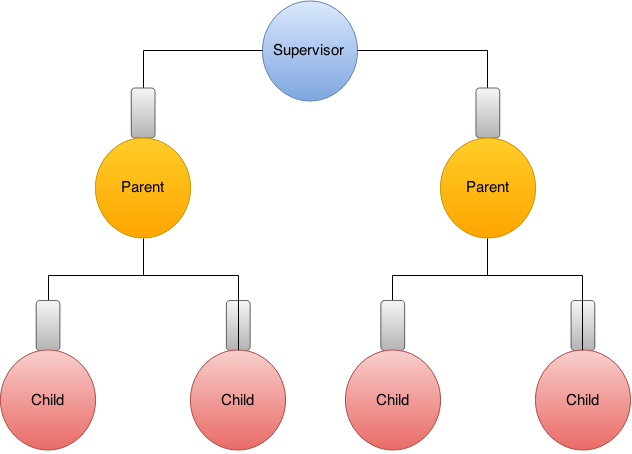
\includegraphics[scale=0.4]{images/tools/ActorModel.png} 
	\caption{Actor Model}
	\label{fig:ActorModel}
\end{figure}
\subsubsection{Actor Model}
The key points of the Actor model is building a hierarchy of  actors that receive messages in their mailbox. Figure \ref{fig:ActorModel} shows the general idea of the actors. The actors have a supervisor that will deliver tasks/messages to their inbox. The actors will then process the messages from their inbox and perform the appropriate task for each message. 
\subsubsection{Akka Actors}
The Actors in Akka are defined by Akka as lightweight, concurrent entities that use an event driven receive loop to process messages in its mailbox. An actors main functions can be boiled down to either receiving or sending messages. Akka's official documentation state that the size of a single actor is 300KB. With 1GB of heap memory, we can create approximately 2.5 million actors. 

These actors may share a thread or operate on different threads. We as developers do not need to worry about this as it is handled by the toolkit.
\\\\
The way the actors determine the appropriate response to a message is by using pattern matching. Pattern matching in short checks if the given message conforms to a certain pattern. This matching can be on the type of the message (int, string, boolean etc.) or on the actual value of the message (1, ``text'', true). By using this we can raise abstraction on how an actor will operate. Pattern matching greatly reduces the clutter that many ``if'' statements can create.
\\\\
Akke also has a feature that enables it to change its state, much like we would expect a protocol to do. It can changes its state to simulate the state of the protocol. This allows us to better understand how our actor will operate through its life cycle.
\begin{figure}[h]
	\centering
	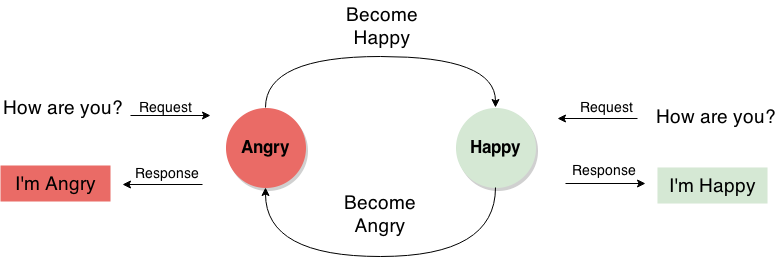
\includegraphics[scale=0.45]{images/tools/ActorState.png} 
	\caption{Actor State showing response to messages}
	\label{fig:ActorState}
\end{figure}
A simple state transition between ``Happy'' and ``Angry'' can be seen in figure \ref{fig:ActorState}. Depending on the state the actor is in, it will respond with a different message. In figure \ref{fig:ActorState} we can see that the response generated from a request is dependent on the state of the actor.

%REF:
%Scala Booker http://www.artima.com/pins1ed/a-scalable-language.html 
%Actor Model http://ieeexplore.ieee.org/xpls/abs_all.jsp?arnumber=886427&tag=1


% ------ Main Content ------
%\section{Architecture}
In this section we have used design by intuition to create the overall architecture of how the system will work. Our argument for doing so is because we lack domain knowledge with using a tool as the one we are about to create. We will only gain this knowledge after we have spent time working on our first implementations of the DSL. Hopefully the development process will guide us to a more defined and fit for purpose architecture.

\subsection{Logical View}
Most of the objectives listed in the Objectives section(p.\pageref{sec:objectives}) are concerned with the ability of implementing the Diffie-Hellman-Merkle key exchange protocol. For our architecture we want to be more general in which protocol we implement. We will focus on creating a foundation for implementing an arbitrary protocol. Afterwards we will see if we need to add or change features to be able to implement a more complex protocol.

\begin{figure}[h]
	\centering
	
\includegraphics[scale=0.45]{images/architecture/ArchitectureFigure1.png} 
	\caption{Logical View of the architecture}
	\label{fig:ArchitectureFigure1}
\end{figure}
Figure \ref{fig:ArchitectureFigure1} shows the overall design for our concept. 
\\
Users must connect through the internet to reach the Consumer. A Consumer is the entity that ''consumes`` the messages\footnote{A message is used to represent a package being sent from one client to the other} that get sent from the Protocol Monitor (PM). A message that goes through the PM must be the expected outcome of the protocol.
\\\\
The PM is drawn as a firewall because it will act in the same way as a firewall does: it has rules that govern what messages are allowed to pass through. The rules contained within the PM will be defined by our DSL.
\\\\
If a message is attempted to be sent or received and it breaks the protocol, the connection is to be terminated. Attempting to repair the connection would in most cases lead to the same error being thrown. Instant termination of the connection would however make both parties aware that the protocol has been broken. There should however be some form of construct that allows for a protocol to branch. This could be added to facilitate the use of multiple versions of a protocol in production.
\\\\
At a later stage we will need to decide at what level the PM ensures that a protocol is obeyed. For simpler protocols we should be able to guaranty full protocol compliance. This becomes much harder to achieve in the case of when a consumer is expecting to receive an encrypted value and that value must have certain properties. For the PM to be able to handle these types of events, it must have the means to decrypt the message.

\subsection{Protocol Monitor}
In order for the architecture to function as we have described, the PM requires certain features. First, it must be able to know if a message received/sent is what the protocol expects. For this to happen the PM must know the state the protocol is in. This state must contain the means of verifying if a new message is expected. The second requirement is that it must be able to act appropriately for the messages received. This includes passing messages along to the users/consumers and also being able to terminate a connection.
\subsubsection{Protocol state}
The task of the PM is to forward and validate messages it receives. For it to validate these messages, it must also contain a state. This state is the state that the defined protocol is in.
\\
Defining the state will be the task of the DSL. Defining such a protocol capable of containing such a fluctuating state needs to be as effortless as possible. The syntax should also be concise so that reasoning about how the protocol operates is obvious.

\subsection{Consumer and Client}
With our definition of what responsibilities the PM has, we can safely assume that all messages successfully sent and received by the consumer and client are valid. In this sense valid means that the message contains a accepted value and is in the correct order.
\subsubsection{Tasks}
The consumer and client must be programmed in such a way that they have handlers that can deal with the messages sent by the other party. They types of messages they receive can be derived directly from the protocol specification. 


\subsection{Mapping}
The task for the Protocol Monitor, Consumer and, optionally, the Client can be all implemented as actors as shown in figure \ref{fig:ArchitectureMapping}. The ``Client'' does not need to be implemented as an actor. Its only requirement is that it must obey the protocol. The Client side could for example be someone using telnet to communicate with the server.
\\
This solution will allow the ``Consumer'' to create additional actors in a hierarchy beneath itself. This would allow for more concurrency and distribute workload and state throughout a system. 
\begin{figure}[h]
	\centering
	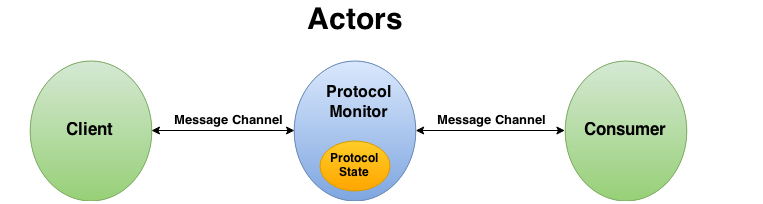
\includegraphics[scale=0.45]{images/architecture/ArchitectureMapping.png} 
	\caption{Representation of our Actors}
	\label{fig:ArchitectureMapping}
\end{figure}

The next part is to be able to define a protocol, the protocol state that the PM will use.























%\subsection{Protocol Monitor -- Add this section to a Solution sec?}
The Protocol Monitor tasks have been described in the previous sections. In this section we will broadly explain how our PM solution works.
\subsubsection{Startup}
To create an instance of a PM we require 3 things, a message channel to communicate with both the client and the consumer and lastly we need the protocol definition. Once the PM has been started, it sends a ``initiation'' message to the consumer. This will allow the consumer to be the one that initiates communication or to initialise certain resources.

\subsubsection{Message forwarding}
When the PM receives a message, it will pattern match and either forward the message to the consumer or client. To distinguish between these we have created two wrapper classes, ``ToConsumer'' and ``ToConnection''. The PM will not read or check the data inside these wrappers, it will only check whether it is a Left or Right value. 
%This is discussed in section \ref{sec:validator} Validator on page \pageref{sec:validator}.
\subsubsection{Ending the connection}
When the client disconnects, we tell the Consumer that we that we are done by sending a ``ConnectionFinished(reason)''. Here the value ``reason'' will represent why the connection ended, either the protocol finished or there was an error.

%Talk about how the PM works... How it communicates with the Connection and Consumer. + Initiation, +ErrorHandling, +Connection shutdown
%

\section{Solution}
\subsection{Defining a protocol}
One possible way of defining a protocol is to use the syntax shown below. This form of syntax is often used when discussing Session Types. They contain the direction of communication and the type of the message. 
$$
\begin{multlined}
Client \Rightarrow Server : Type \\ 
Server \Rightarrow Client : Type \\
end
\end{multlined}
$$
In this protocol the client sends a message to a server. The message that the server receives is to be of a certain type. Examples are: Integers, Strings, Objects etc. After the server has sent its last message, the protocol is over. 
A simple server that simply repeats the messages it receives, an echo server, would be defined in the following way:
$$
\begin{multlined}
Client \Rightarrow Server : String \\ 
Server \Rightarrow Client : String \\
end
\end{multlined}
$$
There is one undesired feature here however. When we reach the end, the connections are closed and we will need to re-establish a connection to send additional messages.
\subsubsection{Looping protocols}
Here we wish to once again implement a echo server. To avoid the user needing to reconnect for each message, we need to provide a way of looping the protocol. One approach would be to have a special case where we tell the protocol to go back to a previously defined step.
$$
\begin{multlined}
Client \Rightarrow Server : String \\ 
Server \Rightarrow Client : String \\ 
goto \rightarrow 0 \\
end
\end{multlined}
$$
When our Protocol Monitor now reaches the ``goto'' step, it should return back to step 0 of the protocol. This solution would however quickly become confusing if the number of goto steps was to increase. It is also not easy to know if the index begins on ``0'' or ``1''.
Also the the definition can become quite verbose when creating longer protocols. Another issue is that the state of both the ``Client'' and ``Server'' is mutated at each line.

\subsubsection{Creating Our Syntax}
In Scala, we can create a syntax that is very similar to the session type syntax shown above. In the following example we will create two end-points, a client and a server. They will be used to define an echo server. First we need to create an instance of a object which has methods for sending, receiving and looping. For this purpose we have created the class ``ProtocolBuilder''. It contains the necessary functions and attributes needed for defining our protocol.
%[style=myScalastyle]
\begin{lstlisting}[style=myScalastyle]
 val client = new ProtocolBuilder()
 val server = new ProtocolBuilder()
\end{lstlisting}
Once they are created, we can begin to define our protocol.
\begin{lstlisting}[style=myScalastyle]
 client send(server, aString)
 server send(client, aString)
 server gotoStep 0
 client gotoStep 0 
\end{lstlisting}
The first obvious change is that we have dropped the arrow syntax in favour of ``send'' and ``receive''. Although Scala can support such operators, it would not improve readability. The second change is that we are not using the type ``String'', but ``aString''. We will discuss this later is section {\ref{sec:validator} Validator}, but for now we will assume that ``aString'' is a validation that checks if the message is a string.   
\\\\
The main concern with this code is that we must define both the client and server side for each send and receive call. In a real implementation, we would only need to focus on one single end-point. By knowing one end of the protocol, we can construct the opposite protocol. In addition, Scala would allow us to omit the parentheses to increase readability, but not when we have two input parameters.
\\\\
Taking the above concerns into consideration, we propose a syntax that avoids this mutability and is less redundant. We have names this syntax the ``ValidProt Syntax'' as is it built around using Validators. 

\subsubsection{ValidProt Syntax -- Better name? Name it at all?}
The following shows the syntax in our DSL for defining a echo client and server.

\begin{lstlisting}[style=myScalastyle]
 val endpoint = new ProtocolBuilder()
 val client  = endpoint sends aString receives aString
 val server  = endpoint receives aString sends aString
\end{lstlisting}
We have removed mutability by making all calls to send or receive return a new instance of a ProtocolBuilder(), this allows us to chain multiple send and receive in one line. This means that the value endpoint is never mutated. With no mutation, we can reuse the endpoint and be assured that it is always a blank starting point for us to use.

To add a loop to the protocol, we add a call to ``looped()'' at the end.
\begin{lstlisting}[style=myScalastyle]
 val client = endpoint send aString receive aString looped()
\end{lstlisting}

Another feature that we have added is that sometimes the order of messages is irrelevant. For example in a chat application, we want the participants to be able to send or receive in any possible order. For allowing this we have implemented the method ``anyone'' that represents sender or receiver is unimportant.

Although protocols are meant to be easy and not contain any complex branching, we have added features that would allow for such protocols.

\subsection{Validator}
\label{sec:validator}
For the task of verifying if a message is of the expected type, we have created a class Validator. Validator is a class that contains a single method, ``validate''. This method contains the logic for testing if a message is of the correct and expected type. ``validate'' signature is the following
\begin{lstlisting}[style=myScalastyle]
    validate: String => Either[ValidationError, Any]
\end{lstlisting}

\begin{description}
 \item[validate] is the name of the method
 \item[String] is the input type for the method
 \item[=>] Given the previous input, return the following
 \item[Either\lbrack Left, Right\rbrack] Either return either a left or right value.
 \item[ValidationError] Left value is of type ValidationError
 \item[Any] Right value is of type Any. Any is, what its name suggest, a type that can return anything.
\end{description}
The main point extract from this definition is the ``Either'' type. For the Either type, a ``Left'' value is considered undesired while the ``Right'' value is the desired one. In our case we set the undesired case to be ValidationError. Validation Error contains two arguments, a String and an optional Exception. The thought is to set the value of the String to an easy to understand message that will tell us what and where something went wrong. The Exception will provide us with the details of what the specific error was. The ``Right'' value allows us to return an ``Any'' type of object. This object will be delivered directly to the Consumer. Implementations of Consumers can then use pattern matching to reason about a protocols state and flow.

To show the simplicity of defining such Validators we will show some examples. First we will create a validator the verifies that a message can be converted to a String. The input of the ''validator`` is a string, so the message must be valid.
\begin{lstlisting}[style=myScalastyle]
  // Return input inside a Right()
  val aString = new Validator(input => Right(input))
  // Wrap input inside Username
  val aUsername = new Validator(input => Right(Username(input)))
\end{lstlisting}
As the input of the validator is a String, that means there is no way the validation can fail or be invalid. This allows us to avoid the need of including a ``Left'' value. To help with pattern matching, we can easily wrap this value inside a class. As shown in the value ``Username'' that wraps a string into a Username object.

We can also create more complex Validators that make more complex evaluation of a message. Here we can check if a message can fulfil the requirements of being a ``special number''.
\begin{lstlisting}[style=myScalastyle]
  val aSpecialNumber = new Validator(input => try {
    val number = input.toInt
    if(isSpecialNumber(number) {
        Right(SpecialNumber(number))
    } else {
        Left("Received message is not a SpecialNumber") 
    }
  } catch {
    case e: Exception =>
      Left(ValidationError("Received message is not an Integer", e) )
  })
\end{lstlisting}
The method ``isSpecialNumber'' does not need to be defined inside the validator. This is because Scala supports closures. They allow us to reference methods or variables outside the current local scope.

\subsubsection{Encrypted Validation}
When a message is encrypted a validator will have no way to determine if it is valid. To do so, it would need to acquire the secret key that can decrypt it. The secret key will only be available from the consumer. To deal with this scenario we, have created a special case class DelayedValidator. DelayedValidator allows us to send a message to the consumer for delayed validation. Once the consumer receives this message it will decrypting the message and pass it back to the Protocol Monitor. The Protocol Monitor will then verify whether the message is correct. The reason for solving the problem this way is to allow the validators to still contain most of the logic of wrapping message to classes. This also provides us with consistency as it is always the PM that handles validation.

   
%Ultimately we will need decide whether we should be able to define conditional steps. For example in the Diffie-Hellman-Merkle protocol, the secure public key must be agreed by both parties. If one client  
%

%loose coupling with protocol. no inheritance

\subsection{Protocol Monitor}
The Protocol Monitor tasks have been described in the previous sections. In this section we will broadly explain how our PM solution works.
\subsubsection{Startup}
To create an instance of a PM we require 3 things, a message channel to communicate with both the client and the consumer and lastly we need the protocol definition. Once the PM has been started, it sends a ``initiation'' message to the consumer. This will allow the consumer to be the one that initiates communication or to initialise certain resources.

\subsubsection{Message forwarding}
When the PM receives a message, it will pattern match and either forward the message to the consumer or client. To distinguish between these we have created two wrapper classes, ``ToConsumer'' and ``ToConnection''. The PM will not read or check the data inside these wrappers, it will only check whether it is a Left or Right value. 
%This is discussed in section \ref{sec:validator} Validator on page \pageref{sec:validator}.
\subsubsection{Ending the connection}
When the client disconnects, we tell the Consumer that we that we are done by sending a ``ConnectionFinished(reason)''. Here the value ``reason'' will represent why the connection ended, either the protocol finished or there was an error.

%Talk about how the PM works... How it communicates with the Connection and Consumer. + Initiation, +ErrorHandling, +Connection shutdown
%





\section{Protocol Implementations}
\subsection{Diffie-Hellman-Merkel}
In this section we will implement a Echo server that uses the Diffie-Hellman-Merkle key exchange to secure the communication channel. The focus of the implementation will not be on the actual encryption of values and strength of keys. We will however focus on how you would create a basic system that can later be expanded. The reason for this is that DHM requires numbers in the size of over 1024 bits to truely be secure. Implementing our solution for this would shift the focus too much on the cryptography aspect rather than the implementation. In  a real world application one would want to use a cryptographic library to handle the generation of these security elements. We have opted to create our own simple methods instead of adding these libraries.

\subsubsection{Specifying the protocol}
The basis of our design will be entirely dependant on the protocol definition. It seems only natural to start the design process here.

\subsubsubsection{JSON}
For this implementation we will use the JSON format for sending and receiving messages. Although our solution can work with any type of message, we find JSON to be easily readable and understandable.
\subsubsubsection{Protocol}
We have written about the Diffe-Hellman-Merkle key exchange in \ref{sec:dhm} Diffie-Hellman-Merkel on page \pageref{sec:dhm}. The key elements of this protocol is Alice starting a communication with Bob by sending a prime Number and generator, message 1. Many real-world implementations use pre-defined generators, but we will allow the generator to be dynamic for our implementation. After Bob receives this message, he sends to Alice his public key. The final step then is for Alice to send her public key. After this the communication can now be encrypted using the key generated by both Alice and Bob.
\\ 
Below we have specified this part of the protocol in our DSL.
\begin{lstlisting}[style=myScalastyle]
 val endpoint = new ProtocolBuilder()
 val aliceDHM = endpoint sends primeAndGenerator 
                  receives aPublicKey sends aPublicKey
 val bobDHM   = endpoint receives primeAndGenerator 
                  sends aPublicKey receives aPublicKey
\end{lstlisting}
The only part missing now is that we want Bob to echo messages sent by Alice. We want Alice to send as many messages as she wants. We have two options to solve this. As the message sent from Alice is encrypted, the validator will not be able to verify the message. Depending on the level of security desired, we can either encrypt the entire message or only the values. To increase clarity in the system, it id beneficial to use the DelayedValidation class. This will help decrease the complexity of the implementation.

\begin{lstlisting}[style=myScalastyle]
 val aliceEcho = endpoint sends anEchoMessage 
                  receives anEchoMessage looped()
 val bobEcho   = endpoint receives anEchoMessage
                  receives anEchoMessage looped()
\end{lstlisting}

Now that we have the two parts of the protocol defined, we can combine them.
\begin{lstlisting}[style=myScalastyle]
 val aliceComplete = aliceDHM next( aliceEcho )
 val bobComplete   = bobDHM next( bobEcho )
\end{lstlisting}
The method ``next'' is a method that allows us to combine two separate ProtocolBuilders. It is useful for when we want to limit the scope of a loop step. In other words the protocol could of been written in a single line by using ``next'' to separate the ``looped()'' step from the DHM steps.
\\
Now we need to create the validators that will be used to verify the messages sent and received.

\subsubsection{Implementing Validators}
From looking at the Protocol specification from the previous section we can determine the classes that are needed. The classes that we create in this section will be sent to the consumer and can be considered as message classes. The consumer will based its response by using pattern matching on the message.
\\
We will not show how to create each class and validator, but show how we could handle the first message of the protocol.
\subsubsubsection{Prime and Generator}
\begin{lstlisting}[style=myScalastyle]
 case class PrimeAndGenerator(prime: Double, generator: Double)
\end{lstlisting}
A ``Case'' class gives us by default an immutable class, ``prime'' and ``generator'' are declared as ``val''s . This is very useful for when we pass messages to our Consumer as it ensures that the message is never mutated while en-route.
\\\\
The JSON representation of this class with the values of (7.0 , 2.0) would be the following:
\begin{lstlisting}[style=myScalastyle]
{
    "type": "PandG",
    "prime": "7.0",
    "generator": "2.0"
}
\end{lstlisting}
In the example below we have used a library that helps us extract JSON information out of a string. 

\begin{lstlisting}[style=myScalastyle]
  val primeAndGenerator = new Validator(input => try {
  val json = parse(input)
  val p = json \ "prime"  
  val g = json \ "generator"
  Right(PrimeAndGenerator(prime = p, generator = g))
  } catch {
    case e: Exception =>
      Left("Msg could not be converted to a 
              PrimeAndGenerator class: " + e.getMessage())
  })
\end{lstlisting}
Here we can see that given any form of exception, we will return a Left value with an error message. Otherwise we will return a Right value with a PrimeAndGenerator instance.

\subsubsection{Consumer}
As we have stated before, the Consumer will use pattern matching when receiving messages. All that is needed to do here is implement a response for each message. In the example below we will not show the details. 
\\
All actors must have a ``Receive'' method that handles received messages. 
\begin{lstlisting}[style=myScalastyle]
def receive = {
    case PrimeAndGenerator(prime, generator) =>
      // Generate our PrivatKey and send it
    case PublicKey(key) =>
      // Calculate the session key
    case EchoMessage(message) =>
      // Return message
    case ProtocolEnded(reason) =>
      // Protocol has ended due to 'reason'
      // Tell PM it is safe to quit
    case _ =>
      // Unknown message received
}
\end{lstlisting}
Shown above is the consumers ``receive'' method that deals with the various message cases. All that is missing from the implementation is calculating the $SecretKey$ and echoing encrypted messages.

\subsection{HTTP Server}
\label{sec:httpserver}
The perhaps most widely used protocol in use today is the HTTP protocol \cite{fielding1999hypertext}. It is mostly used to serve web-pages to browsers. We will in this section create a very simple web server that can serve HTML pages.

\subsubsection{Specifying the protocol}
One of the main difficulties when implementing the HTTP is that unlike our DHM protocol, there is much more information that needs to be wraped in messages. Many of these fields are optional and can be sendt in any order. These optional fields make it much more difficult for us to know what information our consumer will have avaiable when generating a response.

Below we have an example of the fields, HTTP headers are.
\begin{lstlisting}[style=myScalastyle]
  GET / HTTP/1.1
  Host: localhost:8888
  Connection: keep-alive
  Cache-Control: max-age=0
  Accept: text/html
  User-Agent: Mozilla/5.0 (X11; Linux x86_64) AppleWebKit/537.36 (KHTML, like Gecko) Chrome/43.0.2357.81 Safari/537.36
  DNT: 1
  Accept-Encoding: gzip, deflate, sdch
  Accept-Language: en-US,en;q=0.8,no;q=0.6
\end{lstlisting}
Our DSL is able to handle that these fields are optional and allowed to be in any order. The only required field is the ``GET'' line. It conveyes the purpose of the message while the other fields are supplementary information for the request.
\begin{lstlisting}[style=myScalastyle]
val httpServer = endpoint receives RequestHeaders sends 
                           ResponseHeaders 
\end{lstlisting}
Due to time constraints, our server does not run any validation on the ResponseHeaders.
\subsubsection{HTTP server running}
Here we can see the index page of our server. We also provide additional pages such as ``test1'' and ``test2''
\begin{figure}[h]
	\centering
	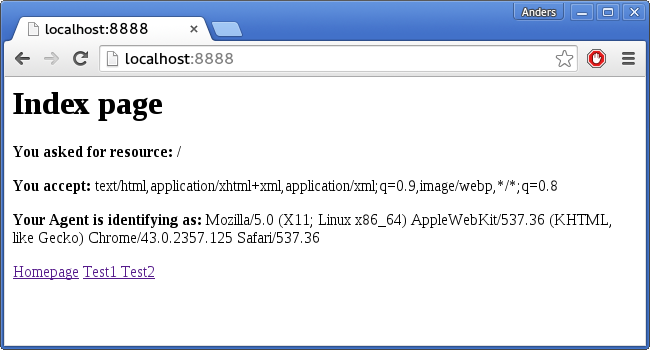
\includegraphics[scale=0.7]{images/protocolimplementations/httpserver.png} 
	\caption{HTTP Server index page}
	\label{fig:httpserver}
\end{figure}

















% ------ End Main Content ------

% Evaluation
\section{Evaluation}
In this section of the paper we will evaluate our work in real world applications and determine its strengths and weaknesses. We will use various implementation to perform this evaluation. We will also look into situations where the implementation does not match the protocol description and observe the systems behaviour.

%\subsection{Test Environment}
%For testing our 
\subsection{Chat Server}
To test the capabilities of our DSL, we decided to create a secure chat application. This application would allow  users to connect to the server and exchange secure and private messages with other connected users. We would establish a secure connection to the server and to each individual user that was connected using the DHM key exchange. This means that our Consumer needs to maintain a list of multiple private session keys and be able to determine which one to use for incoming messages.

One of the key benefits of this solution is that even though our central server will receive all the messages, they will be encrypted using two keys. The first key is the one that is established between the two consumers. The second key is the one that the Server and consumer created. This makes it impossible for the server to know what the actual content of the message is. All the server knows is who is talking to who. 

There will be two parts to a message, the headers and the actual text of the chat message. The headers will determine who the intended recipient is. Below we show an example chat message being sent from A to B.
$$
 \begin{multlined}
  \{\{Headers\}, \{Text\}Key_{A2B}\}Key_{A2Server}
 \end{multlined}
$$
Here we can see that the header is only encrypted with key between consumer A and the Server. The text however is encrypted by both the A2Server and A2B key. When the server receives this message, it decrypts it and forwards it to the correct recipient. It however re-encrypts the message using the B2Server key.
$$
 \begin{multlined}
  \{\{Headers\}, \{Text\}Key_{A2B}\}Key_{B2Server}
 \end{multlined}
$$
\\\\
The steps for the connecting client will be 3 steps. 
\begin{enumerate}
 \item Connect to the server and establish a secure communication channel
 \item Register our Username
 \item Receive and send chat messages
\end{enumerate}

Using the steps shown above we can create the protocol description for the server. 
\begin{lstlisting}[style=myScalastyle]
 val endpoint = new ProtocolBuilder()
 val dhm   = endpoint receives primeAndGenerator 
                  sends aPublicKey receives aPublicKey
 val chatServer = dhm receives aUsername 
                       next endpoint anyone aChatMessage loop()
\end{lstlisting}
Here we have re-used our implementation of DHM we defined earlier and added the messages needed for a chat server.

\subsubsection{Detection of Implementation Errors}
The main purpose of our DSL is to discover errors in implementation. When errors occur, we send the error generated by the Validator to the consumer. These errors will provide us with the information  we need to correct the implementation. 

It is up to the consumer to chose how to handle this error. In our implementation we simply print the error message to the terminal. When we run our application, we will be alerted whenever a error occurs and get the information we need to correct it.

We will show two of the errors we received when we where working on the implementation. One of the errors is when our validation failed. 
\begin{lstlisting}[style=myScalastyle]
  ``ValidationError(Msg could not be converted to a PrimeAndGenerator class: ,net.liftweb.json.MappingException: Do not know how to convert JString(239.0) into double)''
\end{lstlisting}
The first part of the message tells us where the error occurred. The second part is the actual exception that was generated. Using the first message we can see that the error ocurred in the message wrapping for PrimeAndGenerator. The exception tells us that we were unable to map ``JString(239)'' to a Double. This level of detail provides us with more than enough details to correct the error.

The second error we had was when our consumer had not implemented a case for the ``PrimeAndGenerator'' class in its the pattern matching.
\begin{lstlisting}[style=myScalastyle]
  ``Unspecified case for: PrimeAndGenerator(149.0,2.0)''
\end{lstlisting}

As we encounter these errors, we can quickly determine their cause and incrementally fix them until we have a running system. In this case we implemented a case for the PrimeAndGenerator where we continued the process defined in our protocol definition.

\subsubsection{Finished System}
After incrementally adding cases to our consumers pattern matching method, we ended up with a fully functioning system. In our implementation we made the clients chose a random integer as a username when connecting. 

The server alerts connected users when a new users connects. When the connected clients receive this ``NewUser'' alert, they establish a secure connection with the new user and send a simple greeting message. Below we have included the screen-shots of three terminals. The terminals represent the server (\ref{fig:server}), client A (\ref{fig:clienta}) and client B (\ref{fig:clientb}). In this scenario, client A is first to connect to the server and will send a greeting to client B.

\begin{figure}[H]
  \centering
  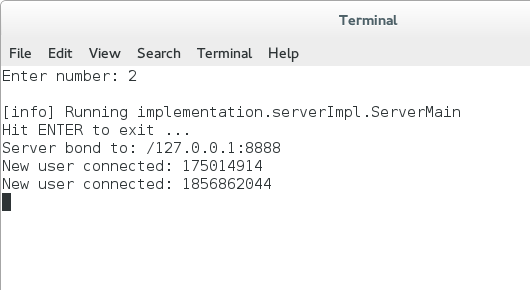
\includegraphics[width=1\linewidth]{evaluation/Server.png}
  \caption{Server}
  \label{fig:server}
\end{figure}

\begin{figure}[H]
  \centering
  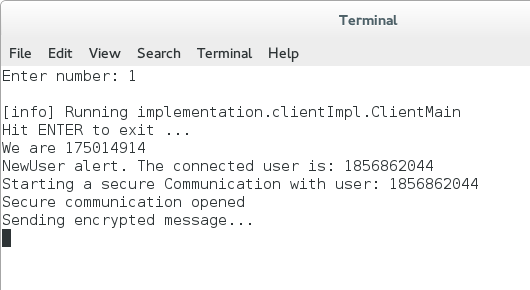
\includegraphics[width=1\linewidth]{evaluation/ClientA.png}
  \caption{Client A - Sends message}
  \label{fig:clienta}
\end{figure}

\begin{figure}[H]
  \centering
  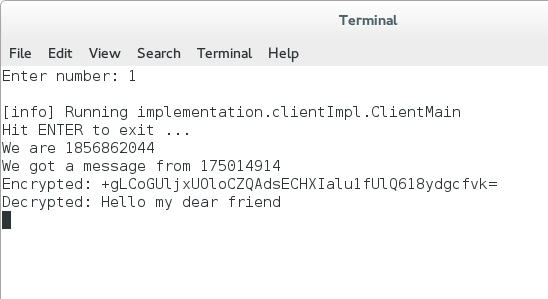
\includegraphics[width=1\linewidth]{evaluation/ClientB.png}
  \caption{Client B - Receives message}
  \label{fig:clientb}
\end{figure}

Any additional clients that connect to the server will also receive greeting messages from both client A and B.

%ServerSide => Unspecified case for: PrimeAndGenerator(149.0,2.0)

%ClientSide => ValidationError(Msg could not be converted to a PrimeAndGenerator class: ,net.liftweb.json.MappingException: Do not know how to convert JString(239.0) into double)


%Server Username => Unspecified case for: LPO2gbvztUktNyx5+BIsidWgBKslDau969BoddEUcs8=

\subsection{Measuring Performance}
To measure the performance of our system, we have decided to implement echo servers that both use and don't use our system.

By using our DSL we will check if every single message sent or received obeys a given protocol. This involves checking that the message contents and protocol specification are of an expected value. These extra steps do not come for free and the overall throughput of the system should be lower than that of a system with no such checking. 

To test this we have created 3 implementations that all build upon the previous implementation. The implementations will be on the server side and will all provide an echo server. The three implementations are the following:

\begin{description}
  \item[Basic] does not use a PM and sends data directly to the consumer
  \item[Uses PM] uses our PM with a simple String Validator
  \item[Wrapping] the Validator wraps messages into an EchoMessage class
\end{description}
We have created a client that measures the time it takes to send and receive a given amount of messages.

The data below shows the average scores for the implementations. As there is some overhead costs when connecting to the server and sending the first message, we do not disconnect and reconnect for each iteration. Instead, we count the time it took to receive the first 10000, 20000, 30000 etc. messages. We gathered results from 20 such iterations. The results below in table \ref{tab:performance} are the averages for each iteration. The time is given in milliseconds. 

\begin{table}[h]
	\centering
	\begin{tabular}{|l|l|l|}
		\hline
		{\bf }         & {\bf Average} & {\bf Message/ms} \\ \hline
		{\bf Basic}    & 489           & 20.40              \\ \hline
		{\bf Uses PM}  & 544           & 18.37              \\ \hline
		{\bf Wrapping} & 589           & 16.37              \\ \hline
	\end{tabular}
	\label{tab:performance}
	\caption{Average performance of implementations given in milliseconds}
\end{table}
% Uses PM is perhaps the most comparable one
If we look at the data we can see quite clearly that there is a performance penalty when using our system. Analysing the performance table we can see that the throughput of the system is reduced by approximately 4 messages in the full implementation that uses wrapping. Sending 10000 round-trip message that bypasses the PM took an average of 489 milliseconds. Messages that went through the PM and were wrapped took on average 589 milliseconds. This is an increase of approximately 20\%. In many application this increase could potentially be unacceptable.

\subsubsection{Concurrency}
One of the objectives was building our DSL so it would be concurrent. To test this we will use the HTTP server we created in sections

\subsubsection{Analysing the performance drop}
The reason why the Basic implementation is faster is that it does not need to read the data it receives. It simply returns whatever it receives, without looking at the contents. The other implementations need to perform several additional steps than just echoing the message:
\begin{enumerate}
  \item Check if receiving is according to the protocol state
  \item Update protocol state
  \item Convert the message to a String 
  \item Validate the message
  \item Send validated message to the Consumer
  \item Generate and send response
  \item Check if sending is according to the protocol state
  \item Validate the message
  \item Update protocol state
  \item Convert message to a ByteString
  \item Send the message
\end{enumerate}
As we can see there are quite a few additional steps involved in our system. It seems only natural that the we would suffer from some form of performance loss.

We feel however that a 20\% cost is acceptable for most applications as we are comparing it to a system that has no checking and does not abide by any type of protocol. In addition, this DSL is not focused on performance, but increasing readability, maintainability and helping with the implementation. If we had more time we could tweak our system to offer better performance, but this was never a high priority during design. 


\subsection{Bug Discovery}
\subsubsection{Performance tests}
While running performance test we stumbled upon what we believed to be a bug inside the DSL itself. After the performance testing client had sent around 70 000 messages to the server, it would have a protocol failure. The error was that the server was receiving a message, while the protocols state was in a sending state. We found this strange as the client only sends a message after it has received a message. As our test client was such a simple implementation, we believed the error was perhaps located somewhere within the DSL.
 
After some debugging of the system, we discovered that the bug was in fact withing the testing client. In our implementation we were accidentally sending an extra message to the server when restarting our counter. After several restarts, the accumulated additional messages would eventually arrive before the server had sent a response.

This error was not discovered when we tested the ``Basic'' implementation, so we had to rerun our performance test for it. This error was only discovered as we were stress testing the system and would most likely not have of been caught if were sending a lower amount of messages.

\subsubsection{Apple's Goto bug}
Apple's goto bug , Formally labeled as ``CVE-2014-1266'' \cite{bland2014finding} is a bug that occurred because of the duplication of a single line of code.  in Apples SSL can be quickly summarized as the error of duplication of a single line of code. This duplicated line of code prevented a security check from being run. A simplified version of the code can be seen below.

\begin{lstlisting}[style=myScalastyle]
if ((err = SecurityCheck1())) != 0)
         goto fail;
         goto fail; // duplicated line
if ((err = SecurityCheck2()) != 0) // dead code
         goto fail;
\end{lstlisting}

This duplicated line causes the ``SecurityCheck2()'' to never be run. The indentation makes it appear to belong to the first ``if'' statement, but the if statement has no curly braces. If statements without curly braces will only include the first line in the if statement.  In this particular case, skipping the final security check would allow for a man-in-the-middle attack.

The actual cause of why this duplicated line was created was most likely due to a merge gone wrong\footnote{Difference of source after merge: \href{https://gist.github.com/hongrich/9176925}{GitHub.com}}. After developers have made changes to the same source file, they will eventually need to combine them. This is often done by merging the two files together. It was highly likely that the duplication occurred in this process.
\begin{figure}[H]
  \centering
  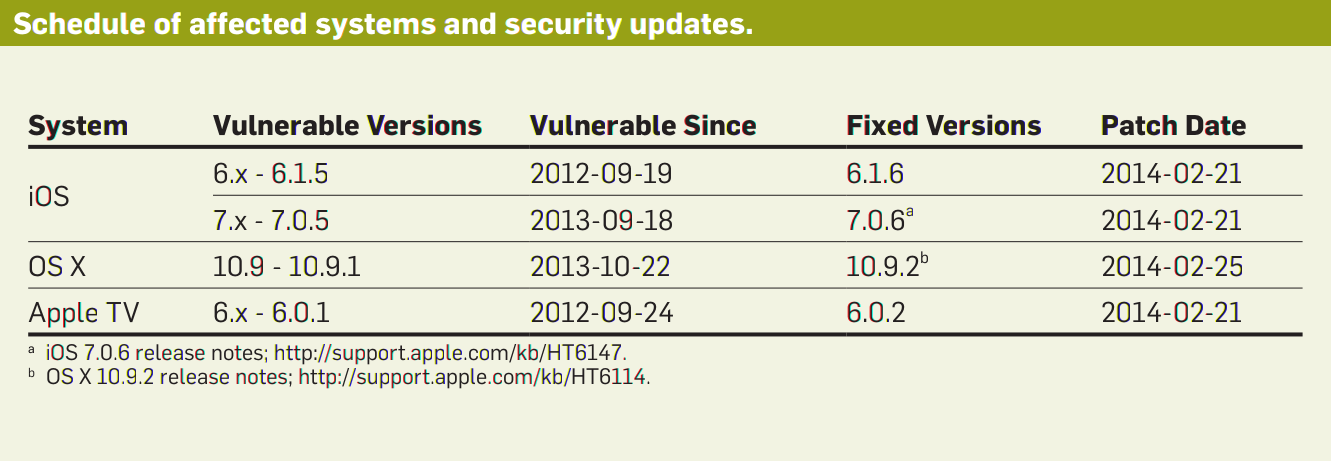
\includegraphics[width=1\linewidth]{evaluation/gotodate.png}
  \caption{Affected systems and patch date of Apple's goto bug \cite{bland2014finding}}
  \label{fig:gotofail}
\end{figure}

There are many questions to how this bug could go unnoticed for so long. In figure \ref{fig:gotofail} we can see that the bug existed for some time before being patched. According to Bland, there are many factors that could of caught this error much sooner:
\begin{itemize}
  \item Coding Standards (indentation, braces)
  \item Code branch merging experience
  \item Code reviews
  \item Coverage data
  \item Compiler warnings
  \item Static analysis warning
  \item Adequate system testing
\end{itemize}

The one that perhaps stands out the most is the fact that the compiler should give a warning when ``dead-code'' is discovered. Dead-code is a term used when a code segment will under no circumstances ever be executed. The SecurityCheck2() should of produced such a warning. Granted you must activate the compiler to show these warnings, but all such errors should always be shown.

The second factor that should of caught this error would be a single unit-test. Landon Fuller has demonstrated that all it would take is 5 lines of code to detect the error\footnote{Landon Fuller's test: \href{https://github.com/landonf/Testability-CVE-2014-1266}{GitHub.com}}.

Bland concludes his article by stating that the error occurred due to a poor development culture within Apple. There are many best practices that they have failed to implement and this resulted in the bug.

Considering the issues described above, I do not believe that the implementation of the Wrapper Syntax would of prevented this bug. It would certainly have of helped as the Validators are easy to use and test-ability. The fact is that the source file that where the bug resides is full of duplicated code. This is something that should of been re-factored during a code review. 

If we assume that the goto bug was included within a Validator, then the Protocol Monitor would not have detected this error. The Protocol Monitor is completely reliant on the implementation of the Validators being correct. If their validate functions contains errors, then the Protocol Monitor will propogate these errors.

%It could of potentially made the error more detectable as the usage of Validators could make testing easier. Apple did however not create a test for their code, even though it would only take 5 lines of code as shown by Fuller. 

Having stated that my system would not have detected Apple's goto bug, I do believe it could of detected similar errors within a different development team. Writing unit tests in general is something that should be done for production ready code. Apple however did not write tests with adequate code coverage and it resulted in this bug. This lead me to agree with Bland conclusion: The root of this bug lies not within the tools used, but rather in the culture of the development team.

\iffalse
\subsubsection{Heartbleed}
Heartbleed\footnote{\href{http://heartbleed.com/}{Heartbleed's Homepage}} was a weakness discovered within the OpenSSL library that would allow for attackers to read the main memory of a system. OpenSSL is an open source cryptographic library for implementing the Secure Socket Layer (SSL) and Transport Layer Security (TLS). It is used by web servers such as Apache and nginx. Data from a web survey\footnote{http://news.netcraft.com/archives/2014/04/02/april-2014-web-server-survey.html}{Netcraft's Web survey}} conducted by Netcraft in 2014, determined that their combined market share was above 60\% when the bug was discovered.

Heartbleed was such a devastating bug as it was a very simple attack, left no traces of an attack and it was a widespread vulnerability. 
\fi


\subsection{Building DSLs with Scala}
Scala is a powerful language that provides us with much freedom in our creation of a DSL. This freedom is however restrictive in certain areas. Many of these restrictions have been discussed in section \ref{sec:scala} Scala.
 
The perhaps most interesting question when evaluating Scala as a host language for a DSL is to ask if it ever got in the way of implementing our DSL the way we wanted to. To answer this question we consider what we would change in our DSL if Scala did not have any restrictions. At the moment of writing, we do not believe that any of the restrictions that Scala has have affected our implementation negatively. If anything our DSL has not taken advantage of the features offered by Scala. Specifically we could use more implicit values and features such as currying \cite{odersky2008programming}. 


\subsection{Weaknesses}
We have identified what we believe to be some of the main weaknesses with this DSL.

The first is the performance loss of approximately 20\%. The performance test was however slightly unfair as the we compared our system to a system with absolutely no wrapping or any data manipulation. We can therefor consider the 20\% loss as the worst case scenario for similar solutions.

The second weakness is specifying protocols that involve more than 2 participants. By using the Event Bus provided by Akka, we are able to enable communication among the consumers, but this communication channel is not necessarily regulated by a Validator. Sending internal messages that are not defined in the protocol specification can cause undesired side-effects. 

A third weakness is that the system provides no constructs for dealing with packet loss in the network. In real work applications packets may travel different paths in the network to reach their target. This means that they can be sent in the correct order, but arrive in an alternative order.

Our final weakness is that there is no indication of error when a consumer should send a message, but is idle. For example, if our echo server does not respond to a echo message, no error would occur. It would only be noticed by the client that would never receive a response. 

%Even though you implement the DSL, there is no guarantee that it will help debugging the implementation. This is because the strengths of this DSL are heavily dependant on the developers and how they decide to implement a network protocol. Although the use of validators provide a clean way of separating concerns in a system, they must be implemented correctly. Poorly written error messages will not provide useful information when debugging. Validators must try to encapsulate as much of the systems complexity as possible. This complexity should be the focus of determining the purpose of a message and wrapping it in a suitable case class. In most cases, the validator should wrap messages inside classes. This will greatly help building the consumers pattern matching function.


\subsection{Accomplished Objectives}
All the objectives have been met, with the exception of the tertiary ones. One of the secondary objective was to be able to implement additional protocols, specifically the Needham-Schroeder protocol. The main difference of this protocol compared to the Diffie-Hellman-Merkel protocol is that it involves direct communication with multiple clients. With our DHM key exchange, HTTP server and chat server implementations, we only have direct communication with a single client.

To solve multiple connections we must use the Event Bus to communicate with the other actors. In Needham-Schroeder we need direct communication with a server and a client. Figure \ref{fig:Needham} shows an example of how we could implement the protocol. 

\begin{figure}[H]
  \centering
  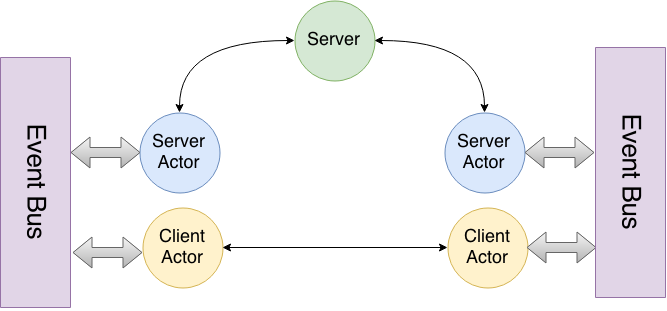
\includegraphics[width=1\linewidth]{evaluation/Needham.png}
  \caption{Needham-Schroeder Actors}
  \label{fig:Needham}
\end{figure}

Here we can create a PM for both the Server and Client actors. This way the PM will be responsible only for communication over a single channel with two participants. The Server and Client actors communicate over the event bus, allowing them to exchange the messages they receive from their connections.

Using similar solutions, we should be able to implement a multitude of different protocols.

 
\iffalse
If you meet your objectives
How did I test it
How do I know its working What happens when it goes wrong
--- Draft 3 ---
How well were the objectives met
What is the performance compared to no checking
-Does not need to quantifiable
How secure it is
How we set out writing it?
"  made this thing using my DSL"
Performance with different message sizes

Speculate on why a sys is slow



Is scala a good language for building a DSL?

This approach definatly has merrits...


Errors: 

ServerSide => Unspecified case for: PrimeAndGenerator(149.0,2.0)

ClientSide => ValidationError(Msg could not be converted to a PrimeAndGenerator class: ,net.liftweb.json.MappingException: Do not know how to convert JString(239.0) into double)


Server Username => Unspecified case for: LPO2gbvztUktNyx5+BIsidWgBKslDau969BoddEUcs8=
\fi


% Conclusion
\section{Conclusion}
In this paper we have explored the various aspects of specifying and implementing network protocols. We have discussed their importance and the difficulties revolved around creating a correct implementation. We have argued that creating a DSL for implementing protocols would be beneficial in managing this complexity.

Our DSL provides a natural way for specifying protocols that help us reason about how one should create implementations. Further we can use this specification to verify that we obey the protocol during run-time. We have showed that the errors generated from the run-time checks provide us with enough information to pin-point exactly what and where something goes wrong. We have also seen that most of the benefits of our DSL relies on its correct usage. This means that developers must dedicate time to specify the message flow of the protocol and create validators for these messages. We have also stated that the Validators must be correct in order for the Protocol Monitor to function. To alleviate this problem we have ensured that testing a validator is a straightforward process.

The usefulness of our DSL has been proven by our implementation of a chat server. This server allows multiple participants to connect and initiate a Diffie-Hellman-Merkel key exchange to establish a secure communication channel to both the server and all connecting clients. Allowing chat participants to exchange messages that only the recipient and sender can decrypt. We have also verified that the actual data being transmitted over the network is encrypted and in the order we have specified. We have also seen that the system is capable of handling a large amount users simultaneously generating requests that must be responded.

The overhead of our solution has been calculated to be around 20\%. A reasonable penalty to be paid for enabling run-time checks. The DSL does still provide its usefulness when performance is the main priority of a system. In these situations we can use the DSL to test a system, not run it. This way we can enable run-time checks on a system while still having the freedom to create the system how ever we desire.

We believe that our solution provides an excellent base for development and implementation of network protocols. It provides a clear advantage in that it also helps create the actual implementation of the protocol, unlike a model checker. It does however not solve all the issues involved with the correct implementation of a protocol. We have examined the case of Apple's Goto bug and seen that it is not a single tool that can solve all problems. Development teams must focus on implementing what are regarded as best practices in software development. Practices such as peer review, testing and coding standards must be in place to reap the full benefit of our system.


\subsection{Future Work}
This paper contains many topics that are worth exploring further. Over the course of this dissertation, we have implemented various protocols and gained a lot of valuable knowledge. Our DSL has seen many changes and new features have been added at an almost consistent pace to solve the problems encountered when implementing new protocols.

Areas that are worth looking into are expanding the DSL to make it more natural when defining validators. The validators are still mostly mostly plain Scala code and use no features of Scala to make it look more like natural language. A great starting point would be to look at the testing framework that we have used to create our own tests, ScalaTest\footnote{\href{http://scalatest.org/}{ScalaTest.org}}. ScalaTest provides a syntax for specifying test cases in a natural language. A test is in reality what a Validators does when it validates an input, so there should be a lot of insight that can be gained from exploring this DSL.

To easier allow for implementing change and allowing new features to be added, our system is not performing to its max potential. It is still in a ``change-friendly'' state where we can make changes without to many consequences. Mainly the state manipulation of the protocol state should be able to perform faster. It would also be interesting to implement the ``Protocol State'' as an actor. In certain cases it should increase performance as well as provide the possibility for additional features.

%After specifying a protocol in our DSL, it would be of great use to be able to generate a model that showed the communication pattern between the participants in the protocol.

%Ideally our DSL would have some form of compile time checks that could check if a consumer had implemented cases for the messages returned from the validators. The compile time errors would then tell us which cases we had not implemented in our consumers. This may not be possible due to the complex nature of the protocol implementation, but is worth researching.


%If given more time we would want to expand our DSL to be able to better monitor the communication over the event bus. Preferably we would want to create a solution where a Protocol Monitor was attached to the event bus, ensuring all communication was regulated by a PM. An alternative approach could be to not rely on the event bus, but allowing the PM to maintain multiple connections, avoiding the need for using the event bus. This may require a complete rework of the DSL, but may be well worth the effort.


%Bibliography
\section{Appendix}
\section*{Appendix A: How to run the Secure Chat Server}
To run the project only one tool is required, Simple Build Tool. SBT can be downloaded and installed from \href{http://www.scala-sbt.org/}{http://www.scala-sbt.org/}

When sbt is installed you need to navigate to the project folder containing ``build.sbt'' and run ``sbt''. This will download all dependencies and start the sbt console. 

Simply type ``run'' inside the sbt console to compile and start the application. There are two main files within the applications that you can start, the Server and Client for the secure chat application. Simply start 3 sbt consols for testing the system. First start the server, then the two clients.

\\\\
The perhaps most interesting source file to look at is the ProtocolBuilder.



\section{Bibliography}

\bibliographystyle{apalike}
\bibliography{bibliographies}


\end{document}
